 \section{Processi Organizzativi}

\subsection{Gestione di processo}

\subsubsection{Scopo}
Secondo lo standard ISO-12207:1995 la gestione di processo contiene le attività e i compiti generici utili per la gestione dei rispettivi processi. Vengono individuate le seguenti attività:
\begin{enumerate}
\item Inizializzazione e definizione dello scopo;
\item Pianificazione e stima dei tempi, delle risorse, dei costi, assegnazione di compiti e responsabilità;
\item Esecuzione e controllo;
\item Revisione e valutazione;
\item Determinazione della fine del processo.
\end{enumerate}

\subsubsection{Obiettivi}
\begin{itemize}
\item Semplificare e gestire la comunicazione tra i membri del gruppo e l'esterno;
\item Coordinare l'assegnazione dei ruoli e compiti;
\item Monitorare il lavoro del gruppo e pianificare le attività da svolgere;
\item Definire le linee guida generali per la formazione dei membri.
\end{itemize}

\subsubsection{Coordinamento}
L'attività di coordinamento è responsabile della gestione delle comunicazioni interne, esterne e delle riunioni.


\paragraph{Comunicazione}
Le comunicazioni avvengono su due piani diversi: tra i membri del gruppo (interno), tra i membri del gruppo e uno o più soggetti esterni (esterno). I soggetti esterni si identificano in:
\begin{itemize}
\item \textbf{Proponente}: l'azienda \textit{Zero12};
\item \textbf{Committenti}:  Prof. \textit{Tullio Vardanega} e Prof. \textit{Riccardo Cardin}.
\end{itemize}

\subparagraph{Comunicazione interna}
I principali mezzi di comunicazione tra membri del gruppo sono: Slack\textsuperscript{G} e Telegram\textsuperscript{G}. 
In particolare, per Slack sono stati creati dei canali appositi per argomenti ed i membri del gruppo dovranno intrattenere le discussioni nei canali ritenuti più appropriati, per evitare confusione e/o ammassi incoerenti di messaggi. La creazione dei canali è stata fatta dal Responsabile di Progetto ed essi saranno destinati a mutare nel tempo per accomodare le esigenze del gruppo.
Telegram viene usato per la componente più informale delle discussioni, per le decisioni meno importanti o in caso di problemi con il funzionamento di Slack (da considerarsi comunque una possibilità remota). 

Per quanto riguarda la comunicazione interna tramite videochiamata (tipicamente le riunioni) lo strumento principale è Discord, scelto poiché semplice, conosciuto da tutti i membri del gruppo e multipiattaforma. In alternativa verrà utilizzato Google Meet o Zoom, entrambi strumenti con i quali tutti i membri del gruppo hanno già avuto esperienza.

\subparagraph{Comunicazione esterna}
Per la comunicazione con i soggetti esterni verrà utilizzato un indirizzo e-mail apposito: \textsl{\href{mailto:dreamteam.unipd@gmail.com}{dreamteam.unipd@gmail.com}} .
Tutti i membri del gruppo avranno accesso alla casella di posta elettronica e saranno tenuti a verificare e notificare il gruppo circa la ricezione di nuovi messaggi, mentre la stesura e l'invio di un nuovo messaggio spetterà al Responsabile di Progetto. Prima dell'invio del messaggio, quest'ultimo sarà sottoposto ad una breve verifica e approvazione da parte del gruppo.
Si sono decise le seguenti convenzioni per quanto riguarda la struttura delle e-mail:
\begin{itemize}
\item L'oggetto dovrà terminare con la dicitura "| SWE - Unipd";
\item In generale il corpo dovrà mantenere un tono il più possibile formale ed il contenuto dovrà essere chiaro e conciso;
\item Il corpo dovrà terminare con la firma "\textit{DreamTeam}".
\end{itemize}

\paragraph{Riunioni}
Le riunione potranno essere interne od esterne. Prima di ogni riunione verrà nominato un segretario che ha lo scopo di far rispettare l'ordine del giorno e dirigere la discussione, tenendo traccia dei punti salienti per poi poter redigere il verbale.

\subparagraph{Riunioni interne}
Alle riunioni interne parteciperanno solo i membri del gruppo, per essere considerate valide dovranno essere presenti almeno quattro dei membri del gruppo. Prima di ogni riunione il Responsabile di progetto dovrà:
\begin{itemize}
\item fissare la data e l'orario;
\item definire l'ordine del giorno;
\item nominare il segretario;
\item comunicare tutto quanto detto sopra (o eventuali variazioni) ai membri con ragionevole anticipo.
\end{itemize}

Gli incontri saranno svolti a cadenza settimanale e, in caso di necessità, anche più frequentemente.
Ogni membro può rivolgersi al Responsabile di progetto per richiedere una riunione interna, proponendo l'ordine del giorno, poi se ritenuta necessaria il Responsabile si attiverà per l'organizzazione dell'incontro.

In ogni caso i membri del gruppo sono liberi di indire riunioni informali tra gli interessati, le persone coinvolte gestiranno orari, date e temi di discussione tra di loro come meglio credono senza intervento del Responsabile di progetto.
Generalmente la riunione non sarà considerata valida e non sarà prodotto un verbale.

\subparagraph{Riunioni esterne}
Alle riunioni esterne parteciperanno sia i membri del gruppo che soggetti esterni (proponente e/o committente). La richiesta di una riunione potrebbe provenire da entrambe le parti (soggetti esterni o Responsabile di progetto) e le piattaforme standard utilizzate saranno GMeet e Zoom, anche se il soggetto esterno è libero di scegliere la piattaforma che più desidera (non sono escluse le riunioni in presenza, se possibili). In ogni caso il Responsabile di progetto dovrà nominare un segretario, incaricato della stesura del verbale.


\subsubsection{Pianificazione}
Secondo lo standard ISO-12207:1995 l'attività di pianificazione prevede la preparazione delle risorse necessarie per l'avvio, l'esecuzione e la gestione di un processo. Spetterà quindi al Responsabile di progetto individuare i materiali, il tempo, il personale e le tecnologie necessarie, verificandone la disponibilità e l'adeguatezza. Parte fondamentale è l'identificazione dei ruoli di progetto e l'assegnazione dei compiti.

\paragraph{Ruoli di progetto}
Vengono identificati 6 ruoli di progetto che i membri dovranno assumere:

\begin{itemize}
\item Responsabile di Progetto;
\item Amministratore di Progetto;
\item Analista;
\item Progettista;
\item Programmatore;
\item Verificatore.
\end{itemize}

Importante notare che ogni membro ricoprirà almeno una volta ogni singolo ruolo e andranno evitati i conflitti di interesse tra ruoli (es. una persona non potrà essere sia redattore che verificatore delle stesse parti)

\subparagraph{Responsabile di progetto}
Il Responsabile di progetto è una figura fondamentale, incaricato di rappresentare il team all'esterno (proponente e committente), di guidare e coordinare il team al raggiungimento degli obiettivi di progetto nel rispetto dei costi e tempi concordati. Sarà un ruolo presente per tutta la durata del progetto.
In particolare il suo ruolo prevede:
\begin{itemize}
\item responsabilità rispetto alle decisioni prese e dei documenti approvati;
\item coordinamento dei membri del team e dei compiti da svolgere;
\item mantenimento delle relazioni del team con i soggetti esterni;
\item valutazione dei rischi e stima dei costi;
\item responsabilità sulla pianificazione nel rispetto delle scadenze e dell'allocazione delle risorse.
\end{itemize}


\subparagraph{Amministratore di progetto}
L'Amministratore di Progetto gestisce e controlla l'ambiente di lavoro, in particolare quelli che sono gli strumenti utilizzati e le regole che il team è tenuto a rispettare per tutta la durata del progetto. Il suo obiettivo è di favorire la produttività dei membri del gruppo. Generalmente presente per tutta la durata del progetto.
I compiti specifici di questa figura sono:
\begin{itemize}
\item definire le norme e le procedure alla base del lavoro;
\item regolare le infrastrutture e i servizi utili per lo svolgimento dei processi ;
\item gestire il versionamento dei prodotti e la loro configurazione;
\item individuare strumenti utili a migliorare e/o automatizzare i processi;
\item gestire la documentazione di progetto.
\end{itemize}

\subparagraph{Analista}
L'Analista è un ruolo fondamentale che partecipa al progetto soprattutto nella fase iniziale, con lo scopo di comprendere appieno e semplificare il problema, riducendolo ai suoi concetti chiave.
I suoi compiti sono:
\begin{itemize}
\item studiare e definire il problema;
\item identificare quali sono i vari bisogni e richieste, dalla quale saranno estratti dei requisiti;
\item redigere l'analisi dei requisiti.
\end{itemize}

\subparagraph{Progettista}
Il Progettista ha il compito di produrre una soluzione che soddisfi il problema e i bisogni individuati dagli analisti nell'Analisi dei Requisiti.
I suoi compiti sono:
\begin{itemize}
\item sviluppare una soluzione che rispetti tutti e soli i requisiti individuati;
\item produrre un'architettura adatta, in coerenza con i bisogni da soddisfare, che sia affidabile e consistente;
\item perseguire il più possibile efficienza e riusabilità;
\item impegnarsi a rimanere nei costi prestabiliti.
\end{itemize}


\subparagraph{Programmatore}
Il Programmatore è responsabile della codifica e si occupa di implementare l'architettura sviluppata dal Progettista.
In particolare deve:
\begin{itemize}
\item produrre codice che sia il più possibile orientato alla futura manutenzione, versionabile e documentato;
\item scrivere il manuale utente per il codice prodotto.
\end{itemize}

\subparagraph{Verificatore}
Il Verificatore ha il ruolo di controllare ciò che viene prodotto dagli altri membri del team.
In particolare deve:
\begin{itemize}
\item controllare e individuare eventuali errori del prodotto in esame (fase di revisione);
\item segnalare eventuali errori all'autore (o al responsabile) del prodotto analizzato.
\end{itemize}


\paragraph{Gestione dei ticket}
La gestione dei ticket\textsuperscript{G} è un'attività fondamentale in quanto serve al Responsabile di Progetto per assegnare i vari compiti ai membri del team, mentre permette a quest'ultimi di gestire meglio il carico di lavoro, mostrando anche la progressione del progetto.

Il servizio di ticketing scelto è quello offerto da GitHub\textsuperscript{G}, tramite le issue\textsuperscript{G}. Il motivo principale di questa decisione è la comodità della piattaforma, già conosciuta dalla maggioranza dei membri del gruppo, evitando l'introduzione di strumenti aggiuntivi.

\begin{figure}[!h]
\centering
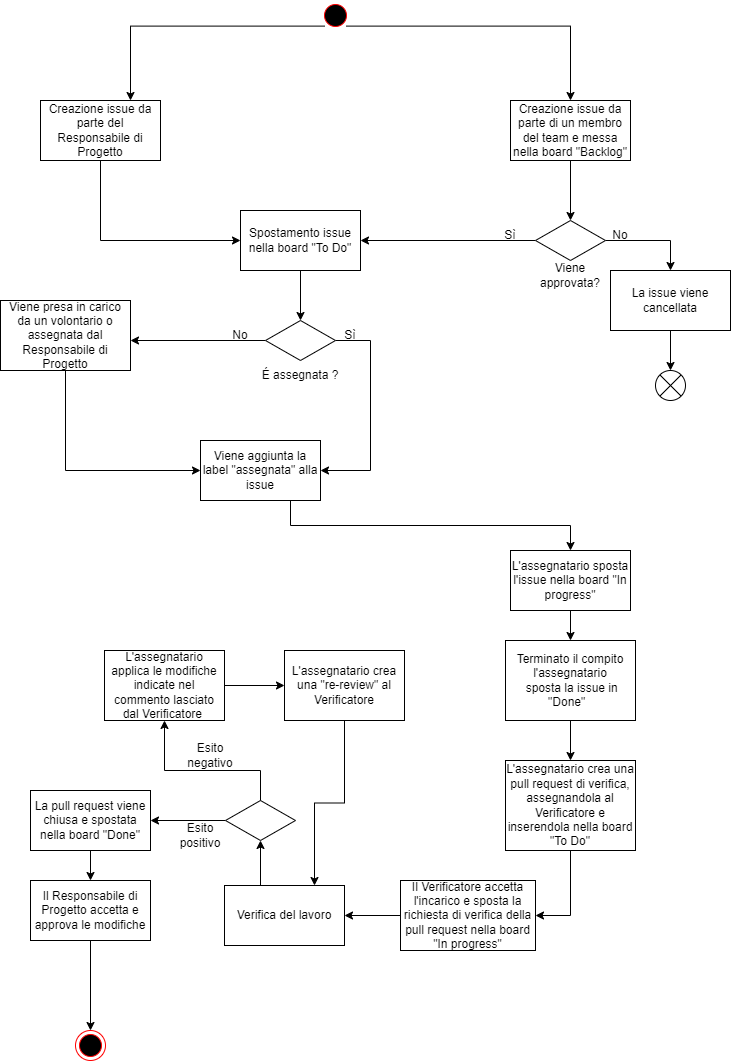
\includegraphics[scale=0.5]{Contenuto/Immagini/ticket.png}
\caption{Attività di gestione dei ticket}
\end{figure}

Note:
\begin{itemize}
\item Viene data a tutti i membri la possibilità di proporre un ticket per snellire la procedura;
\item Il Responsabile di Progetto può decidere di scomporre un ticket in "sotto-ticket" quando ritiene che questo sia troppo complesso;
\item In generale i membri sono tenuti a dare titoli e descrizioni concise e coerenti dei ticket che creano, non saranno accettati ticket con corpo vuoto o ticket senza scadenza;
\end{itemize}

\paragraph{Metriche}
Le metriche adottate per la valutazione del processo di pianificazione sono le seguenti:
\begin{itemize}
\item \textbf{MPC02 Budgeted cost of work scheduled};
\item \textbf{MPC03 Actual cost of work performed};
\item \textbf{MPC05 Schedule variance};
\item \textbf{MPC06 Budget variance}.
\end{itemize} 
Per maggiori informazioni consultare l'appendice B.

\paragraph{Strumenti}
Per il supporto all’attività di pianificazione di progetto è stato scelto come strumento
\textbf{GanttProject}, software open-source e multi-piattaforma usato per la realizzazione di diagrammi di Gantt. Servirà per tenere traccia dell'assegnazione delle risorse, del rispetto delle scadenze e dell'analisi dei carichi di lavoro.


\subsection{Formazione dei membri del team}
Il processo di formazione ha lo scopo di assicurare che ogni membro abbia le conoscenze necessarie per svolgere i compiti che gli vengono assegnati e deve garantire il mantenimento di un personale competente nel tempo.

\subsubsection{Obiettivi}
Il processo mira al mantenimento costante (auspicabilmente per tutta la durata del progetto) di membri competenti ed esperti e garantisce quindi qualità di lavoro in linea con le aspettative.

\subsubsection{Formazione interna}
Ogni membro dovrà provvedere alla propria formazione in maniera autonoma, approfondendo le proprie mancanze con lo studio personale. I membri più esperti potranno condividere le loro conoscenze e/o materiale con il resto del team. In ogni momento un membro che trova difficoltà nell'esecuzione di un compito può rivolgersi al Responsabile di Progetto che dovrà organizzare le attività necessarie per l'apprendimento. Si farà riferimento alla documentazione seguente, ma essendo non esaustiva è consigliato un approfondimento con materiale reperito di proprio conto:
\begin{itemize}
\item \textbf{\LaTeX}: \mylink{https://www.latex-project.org/help/documentation/};
\item \textbf{GitHub}: \mylink{https://docs.github.com/};
\item \textbf{Git}: \mylink{https://git-scm.com/doc};
\item \textbf{Node.js} \textsuperscript{G}: \mylink{https://nodejs.org/api/};
\item \textbf{AWS Cognito}\textsuperscript{G}: \mylink{https://docs.aws.amazon.com/cognito/latest/developerguide/};
\item \textbf{AWS Comprehend}\textsuperscript{G}: \mylink{https://docs.aws.amazon.com/comprehend/};
\item \textbf{API Gateway}\textsuperscript{G}: \mylink{https://docs.aws.amazon.com/apigateway/latest/developerguide/};
\item \textbf{AWS Lambda}\textsuperscript{G}: \mylink{https://docs.aws.amazon.com/lambda/}.
\end{itemize}

\subsubsection{Formazione esterna}
L'azienda proponente zero12 ha deciso di offrire ai membri del team una formazione specifica sulle tecnologie da loro richieste. L'azienda fornirà di volta in volta risorse informative sul canale Slack apposito, con lo scopo di fornire già una minima preparazione prima degli incontri formativi. Ogni membro è tenuto ad uno studio personale del materiale condiviso prima di ogni incontro.


\subsubsection{Strumenti a supporto della gestione organizzativa}
Il team userà i seguenti strumenti per supportare il processo di gestione organizzativa:
\begin{itemize}
\item \textbf{Slack}: strumento standard usato dal team per la comunicazione interna e con il proponente;
\item \textbf{Telegram}: strumento di messaggistica usato dal team per decisione e questioni meno importanti; 
\item \textbf{Git}: strumento utilizzato per il versionamento;
\item \textbf{GitHub}: strumento utilizzato per il versionamento e per il salvataggio di tutti i file prodotti dai membri del team; 
\item \textbf{GitHub Issues}: sistema integrato in GitHub usato per la gestione dei ticket;
\item \textbf{Google Drive}: utilizzato per la condivisione di documenti che richiedono molti cambiamenti dove la modifica in tempo reale è richiesta;
\item \textbf{Gmail}: servizio di posta elettronica scelto dal gruppo;
\item \textbf{Zoom}: strumento usato all'inizio per fare riunioni tra membri del team;
\item \textbf{Discord}: strumento standard usato per le riunioni tra i membri del team. 
\end{itemize}
